\documentclass[aspectratio=169, 11pt]{beamer}

% ============================================
% THEME AND APPEARANCE
% ============================================

\usetheme{metropolis}
\usecolortheme{default}

% Custom colors
\definecolor{darkblue}{RGB}{0, 51, 102}
\definecolor{oxfordblue}{RGB}{0, 33, 71}
\definecolor{lightgray}{RGB}{245, 245, 245}
\definecolor{accentred}{RGB}{166, 25, 46}

\setbeamercolor{frametitle}{bg=darkblue, fg=white}
\setbeamercolor{title}{fg=darkblue}
\setbeamercolor{structure}{fg=darkblue}
\setbeamercolor{alerted text}{fg=accentred}

% Remove navigation symbols
\setbeamertemplate{navigation symbols}{}

% Frame numbers
\setbeamertemplate{footline}[frame number]

% ============================================
% PACKAGES
% ============================================

\usepackage{graphicx}
\usepackage{booktabs}
\usepackage{tikz}
\usepackage{pgfplots}
\pgfplotsset{compat=1.17}
\usepackage{hyperref}
\usepackage{appendixnumberbeamer}

% ============================================
% TITLE PAGE
% ============================================

\title{\textit{How Progress Ends} \\ by Carl Benedikt Frey}
\subtitle{European Economic History --- Spring 2026}
\author{Richard Schulz \and Paula Gradu}
\institute{University of California, Berkeley \\ with Barry Eichengreen}
\date{April 2026}

\begin{document}

% ============================================
% TITLE SLIDE
% ============================================

\begin{frame}[plain]
    \titlepage
\end{frame}

% ============================================
% ROADMAP
% ============================================

\begin{frame}{Roadmap}
    \begin{enumerate}
        \item About the author --- is a book the right venue?
        \item The central thesis
        \item China's reversal of fortune
        \item Europe's decentralized advantage
        \item Paths to industrialization: Britain, Germany, Russia, Japan, America
        \item Cold War divergence and modern stagnation
        \item Critical assessment
        \item Discussion
    \end{enumerate}

    \vspace{1em}
    \textit{Second half: Q\&A with the author}
\end{frame}

% ============================================
% ABOUT THE AUTHOR
% ============================================

\begin{frame}{About the Author: Carl Benedikt Frey}
    \begin{columns}
        \begin{column}{0.65\textwidth}
            \begin{itemize}
                \item Dieter Schwarz Associate Professor, Oxford Internet Institute
                \item Director of the Future of Work programme, Oxford Martin School
                \item Previously: \textit{The Technology Trap: Capital, Labor, and Power in the Age of Automation} (2019)
                \item Research focus: economics of AI, technological change, and labor markets
                \item Ph.D. in Economic History
                \item Frequent contributor to policy debates on automation and inequality
            \end{itemize}
        \end{column}
        \begin{column}{0.3\textwidth}
            \begin{center}
                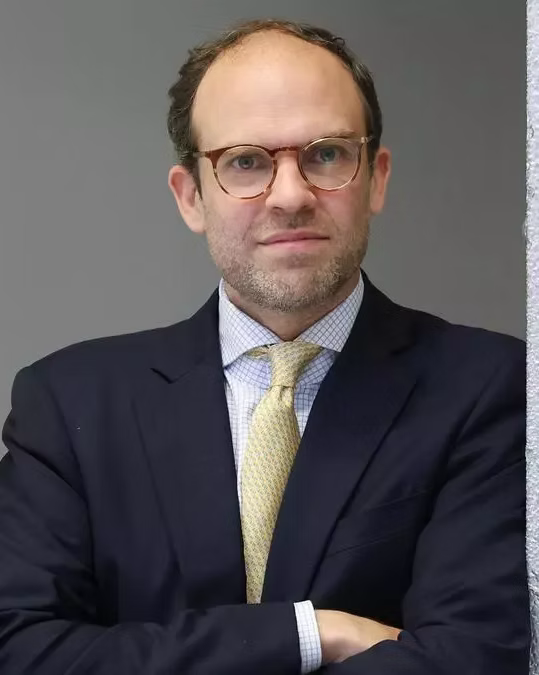
\includegraphics[width=\textwidth]{frey.png}
            \end{center}
        \end{column}
    \end{columns}

    \vspace{0.5em}
    \small Oxford University Press, February 2025 --- 378 pages
\end{frame}

% ============================================
% WHY A BOOK?
% ============================================

\begin{frame}{Is a Book the Right Venue?}
    \begin{columns}[T]
        \begin{column}{0.48\textwidth}
            \textbf{What the format enables:}
            \begin{itemize}
                \item Sweeping narrative across 2,000+ years
                \item Synthesizes growth theory, political economy, history of science
                \item Accessible beyond academia
            \end{itemize}
        \end{column}
        \begin{column}{0.48\textwidth}
            \textbf{What it sacrifices:}
            \begin{itemize}
                \item No formal model --- mechanism never precisely defined
                \item Evidence is illustrative, not causal
                \item Hard to falsify: which cases would \textit{disprove} the thesis?
                \item Selection of episodes may confirm the prior
            \end{itemize}
        \end{column}
    \end{columns}

    \vspace{1em}

    \begin{center}
        \textit{Could the core claims have been a series of papers instead?}
    \end{center}
\end{frame}

% ============================================
% CENTRAL THESIS
% ============================================

\begin{frame}{The Central Thesis}
    \begin{center}
        \Large
        Technological progress is not automatic. \\[0.5em]
        It depends on \textbf{institutions} --- specifically, the balance \\
        between \alert{centralization} and \alert{decentralization}.
    \end{center}

    \vspace{1em}
    \pause

    \begin{itemize}
        \item \textbf{Decentralization} $\rightarrow$ experimentation, autonomy, frontier innovation
        \item \textbf{Centralization} $\rightarrow$ scaling, catch-up growth, imitation
        \item Neither extreme works alone; the \textit{balance} matters
    \end{itemize}

    \pause
    \vspace{0.5em}

    \begin{block}{Core claim}
        Societies that centralize too much stifle the exploration needed for breakthrough innovation. Progress can --- and has --- ended before.
    \end{block}
\end{frame}

\begin{frame}{The Framework: Exploration vs.\ Exploitation}
    \begin{columns}
        \begin{column}{0.48\textwidth}
            \textbf{Exploration} \\
            (Decentralized)
            \begin{itemize}
                \item Trial and error
                \item Autonomous agents
                \item Frontier innovation
                \item High variance, high upside
                \item Markets, federalism, universities
            \end{itemize}
        \end{column}
        \begin{column}{0.48\textwidth}
            \textbf{Exploitation} \\
            (Centralized)
            \begin{itemize}
                \item Scaling known solutions
                \item Top-down coordination
                \item Catch-up growth
                \item Efficient but rigid
                \item Bureaucracies, state planning
            \end{itemize}
        \end{column}
    \end{columns}

    \vspace{1em}
    \pause

    \begin{center}
        \textit{Key insight:} Countries at the technological \textbf{frontier} need exploration; \\
        countries \textbf{behind} the frontier can grow via exploitation --- but only temporarily.
    \end{center}
\end{frame}

\begin{frame}{Contrast: Greif, Mokyr \& Tabellini, \textit{Two Paths to Prosperity}}
    \small
    \textbf{Shared ground:}
    \begin{itemize}
        \item Both compare Europe and China over the long run (1000--2000)
        \item Both reject simple ``Europe was better'' narratives
        \item Both emphasize political fragmentation as key to Europe's divergence
    \end{itemize}

    \vspace{0.5em}

    \textbf{Where they diverge:}
    \begin{itemize}
        \item \textbf{GMT:} Europe's fragmentation $\rightarrow$ warfare $\rightarrow$ fiscal-military states $\rightarrow$ capital-intensive growth. China's unity $\rightarrow$ peace $\rightarrow$ labor-intensive, Smithian growth. \textit{Two viable paths}, not one failure.
        \item \textbf{Frey:} Fragmentation $\rightarrow$ innovation. Centralization $\rightarrow$ stagnation. More normatively loaded --- one path ultimately wins at the frontier.
    \end{itemize}

    \vspace{0.3em}
    \begin{center}
        \textit{Does Frey's framework undervalue the Smithian growth path?}
    \end{center}
\end{frame}

% ============================================
% CHINA
% ============================================

\begin{frame}{The Needham Puzzle: Why Did China Fall Behind?}
    \textbf{China's early lead:}
    \begin{itemize}
        \item Bureaucratic state from 221 BC (Qin unification)
        \item Printing, gunpowder, compass, paper --- centuries before Europe
        \item Civil service examinations from 605 AD
        \item Song dynasty (960--1279): ``an industrial revolution that almost was''
    \end{itemize}

    \pause
    \vspace{0.5em}

    \textbf{What went wrong?}
    \begin{itemize}
        \item \alert{Political unity} eliminated interstate competition
        \item The exam system channeled talent into bureaucracy, not innovation
        \item Ming sea ban (1371): shut down maritime exploration
        \item Patronage economy under Qing: loyalty $>$ innovation
    \end{itemize}
\end{frame}

\begin{frame}{China: The Fiscal Capacity Trap}
    \begin{columns}[T]
        \begin{column}{0.48\textwidth}
            \textbf{Frey's key evidence:}
            \begin{itemize}
                \item Tax revenue per capita \textit{declined} from Song to Qing
                \item By 1900, China's fiscal capacity was a fraction of Europe's
                \item A vast empire with a surprisingly weak state
            \end{itemize}

            \vspace{0.5em}
            \pause

            \textbf{The paradox:}
            \begin{itemize}
                \item Centralized enough to \textit{block} innovation from below
                \item Too weak to \textit{invest} in modernization from above
            \end{itemize}
        \end{column}
        \begin{column}{0.48\textwidth}
            \begin{center}
                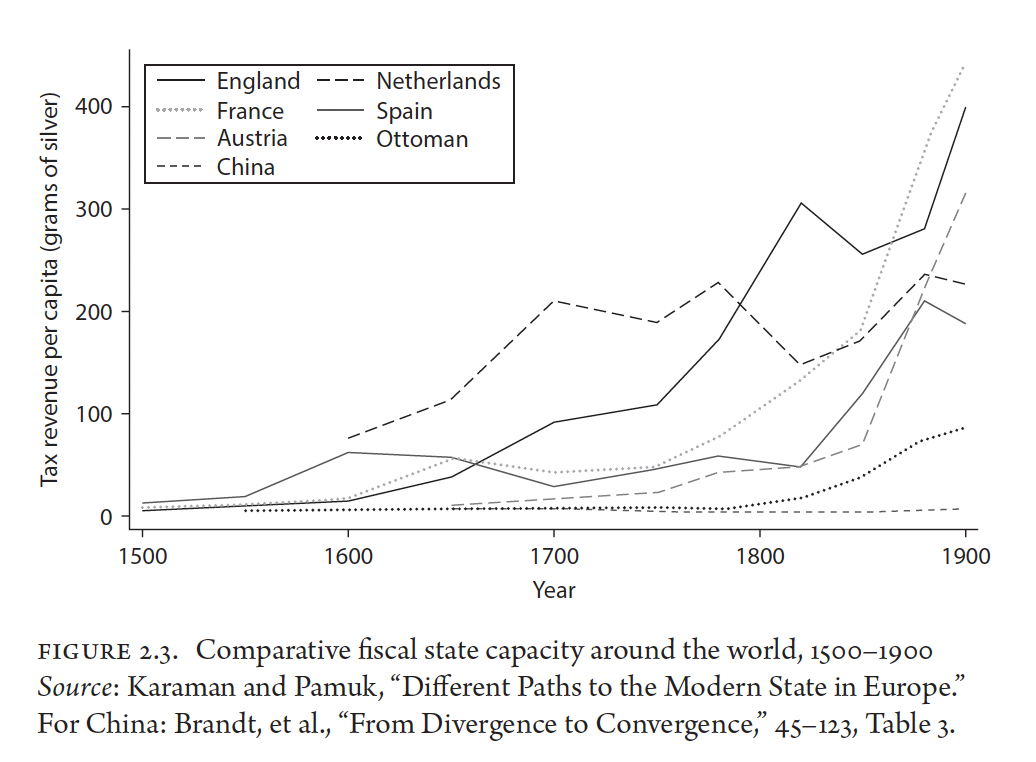
\includegraphics[width=\textwidth]{fig2.3.png}
            \end{center}
        \end{column}
    \end{columns}
\end{frame}

% ============================================
% EUROPE
% ============================================

\begin{frame}{The Rise of Europe: Decentralization as Engine}
    \textbf{Why Europe?} The fall of Rome \textit{enabled} progress.

    \vspace{0.5em}

    \begin{itemize}
        \item \textbf{Political fragmentation:} Hundreds of competing polities
        \item \textbf{Germanic traditions:} Assemblies, consensual governance
        \item \textbf{Parliaments:} Le\'{o}n (1188), Magna Carta (1215) --- constraints on rulers
        \item \textbf{Communes:} Self-governing cities (Italian city-states, Hanseatic League)
        \item \textbf{The Church:} Banned cousin marriage $\rightarrow$ weakened clans $\rightarrow$ strengthened individualism and voluntary associations
    \end{itemize}

    \vspace{0.5em}
    \begin{block}{Key mechanism}
        Interstate competition + exit options for talent $\rightarrow$ rulers had to offer good institutions to attract productive people.
    \end{block}
\end{frame}

\begin{frame}{Britain: The Model of Decentralized Innovation}
    \begin{itemize}
        \item Glorious Revolution (1688): parliamentary sovereignty, property rights
        \item Patent system: credible commitment to protect inventors
        \item No guilds monopolizing knowledge; artisan-driven experimentation
        \item Industrial Revolution as \textit{bottom-up} phenomenon
    \end{itemize}

    \vspace{1em}
    \pause

    \textbf{Frey's interpretation:}
    \begin{itemize}
        \item Britain succeeded not because of a strong state directing innovation\ldots
        \item \ldots but because the state \textit{could not} easily block innovators
        \item Parliament represented merchant/industrial interests
        \item Creative destruction was politically tolerated
    \end{itemize}
\end{frame}

% ============================================
% PATHS TO INDUSTRIALIZATION
% ============================================

\begin{frame}{Germany/Prussia: Bureaucratic State Capitalism}
    \begin{itemize}
        \item Frederick the Great's bureaucratic reforms: meritocratic, efficient
        \item \textbf{Education first:} Prussia built mass schooling \textit{before} industrialization --- the reverse of Britain, where industry drove education demand
        \item State-directed industrialization: railroads, steel, chemicals
        \item \textbf{Universities:} Humboldt model --- research universities with genuine autonomy
        \item German universities dominated Nobel Prizes until 1933
    \end{itemize}

    \vspace{0.5em}
    \pause

    \textbf{The catch:}
    \begin{itemize}
        \item Worked brilliantly for \textit{catch-up} (replicating British innovations)
        \item State coordination scaled applied science effectively
        \item But: when regime changed to Nazi control, university autonomy collapsed
        \item Brain drain (Einstein, Fermi, von Neumann\ldots) $\rightarrow$ US inherited the frontier
    \end{itemize}
\end{frame}

\begin{frame}{Russia and Japan: Imitation Without Exploration}
    \begin{columns}[T]
        \begin{column}{0.48\textwidth}
            \textbf{Russia/USSR}
            \begin{itemize}
                \item Weak state \textit{and} weak society
                \item Serfdom until 1861
                \item Central planning as ``exploitation machine''
                \item Impressive catch-up (steel, space)
                \item Virtually zero breakthrough inventions
            \end{itemize}
        \end{column}
        \begin{column}{0.48\textwidth}
            \textbf{Japan}
            \begin{itemize}
                \item Meiji state-led modernization
                \item Pilot factories $\rightarrow$ privatized to zaibatsu
                \item Labor repression funded capital accumulation
                \item Caught up fast, but breakthrough inventions: negligible
            \end{itemize}
        \end{column}
    \end{columns}

    \vspace{0.5em}

    \begin{center}
        \textit{``To paraphrase one scholar, if Japan's experience teaches any single lesson, it is that myriads of simple improvements to established technologies can take a country a long way.''}
    \end{center}
\end{frame}

\begin{frame}{America: The Innovation Powerhouse}
    \textbf{Why the US took the lead:}
    \begin{itemize}
        \item \textbf{Federalism:} States as ``laboratories of democracy'' (Brandeis)
        \item \textbf{Constitution:} Patent clause enshrined innovation incentives from 1787
        \item \textbf{Democratic innovation:} Broad-based patenting, not just elites
        \item \textbf{Frontier individualism:} Geographic mobility, weak guilds
        \item \textbf{ARPA model:} Decentralized funding, high autonomy for researchers
    \end{itemize}

    \vspace{0.5em}
    \textbf{Key contrast with Europe:}
    \begin{itemize}
        \item US patent holders were far more socially diverse
        \item Innovation was not a preserve of the educated elite
        \item ``Democratized'' invention $\rightarrow$ more experimentation
    \end{itemize}
\end{frame}

\begin{frame}{ARPA and the Internet: Decentralized Innovation in Practice}
    \textbf{The ARPA model} (est.\ 1958):
    \begin{itemize}
        \item Small agency, flat hierarchy, program managers with high autonomy
        \item Funded high-risk research with no immediate commercial application
        \item Trusted researchers to define problems, not just solve assigned ones
    \end{itemize}

    \vspace{0.5em}

    \textbf{The Internet as case study:}
    \begin{itemize}
        \item ARPANET (1969): designed for resilience, not central control
        \item Open protocols (TCP/IP) enabled permissionless innovation
        \item No single firm or government directed the web's development
        \item Result: the most consequential innovation platform of the 20th century
    \end{itemize}

    \vspace{0.5em}
    \begin{center}
        \textit{Frey's strongest example: state funding + decentralized execution = breakthrough.}
    \end{center}
\end{frame}

% ============================================
% COLD WAR AND MODERN STAGNATION
% ============================================

\begin{frame}{Cold War: The Great Experiment}
    \begin{center}
        \textbf{USSR vs.\ China after 1949: Two paths of communism}
    \end{center}

    \vspace{0.5em}

    \begin{columns}
        \begin{column}{0.48\textwidth}
            \textbf{Soviet Union}
            \begin{itemize}
                \item Rigid central planning
                \item \textit{Nomenklatura} system: political loyalty over competence
                \item Khrushchev's Sovnarkhoz reform failed
                \item Stagnation by 1970s
            \end{itemize}
        \end{column}
        \begin{column}{0.48\textwidth}
            \textbf{China (post-1978)}
            \begin{itemize}
                \item Deng's \textit{gradual} reforms
                \item Regional decentralization
                \item Special Economic Zones (Shenzhen)
                \item ``Crossing the river by feeling the stones''
            \end{itemize}
        \end{column}
    \end{columns}

    \vspace{0.5em}
    \pause

    \textbf{Frey's reading:} China's success was \textit{decentralization within an autocracy} --- but this has limits\ldots

    \vspace{0.3em}
    \begin{center}
        % \includegraphics[width=0.5\textwidth]{figures/fig10_2_gdp_ussr_china.pdf}
        \textit{[Fig.\ 10.2: GDP per capita, USSR vs.\ China, 1920--2010]}
    \end{center}
\end{frame}

\begin{frame}{The Dictator's Dilemma}
    \begin{center}
        \Large
        Autocrats \textbf{need} innovation for legitimacy and power, \\
        but \textbf{fear} the autonomy innovation requires.
    \end{center}

    \vspace{1em}
    \pause

    \begin{itemize}
        \item Innovation requires free information flows --- but these threaten regime control
        \item Autonomous researchers may produce politically inconvenient truths
        \item Successful entrepreneurs become independent power centers
        \item Xi Jinping's recentralization: crackdowns on tech firms, universities, SEZs
    \end{itemize}

    \vspace{0.5em}
    \pause

    \begin{block}{Historical parallel}
        Ming China, Nazi Germany, late USSR --- all centralized at the cost of innovation.
    \end{block}
\end{frame}

\begin{frame}{Modern Stagnation: Not Just China}
    \textbf{Frey argues the US faces its own innovation slowdown:}

    \begin{itemize}
        \item Declining research productivity (more researchers, fewer breakthroughs)
        \item University bureaucratization: compliance, administration, risk aversion
        \item Regulatory accumulation: harder to experiment (pharma, energy, construction)
        \item Geographic sorting: innovation concentrated in fewer places
        \item Political polarization undermining institutional trust
    \end{itemize}

    \vspace{0.5em}

    \begin{center}
        \alert{The ``veneer of progress'':} We may be coasting on past \\ institutional investments while the foundations erode.
    \end{center}
\end{frame}

% ============================================
% EPILOGUE: AI AND MORAVEC'S PARADOX
% ============================================

\begin{frame}{Epilogue: AI and Moravec's Paradox}
    \textbf{Moravec's Paradox:}
    \begin{itemize}
        \item Computers excel at tasks humans find hard (calculation, chess)
        \item But struggle with tasks humans find easy (perception, physical manipulation)
    \end{itemize}

    \vspace{0.5em}
    \pause

    \textbf{Frey's provocation:}
    \begin{itemize}
        \item AI is extremely good at \textit{exploitation} --- pattern recognition, optimization
        \item But genuine \textit{exploration} --- creative leaps, paradigm shifts --- remains elusive
        \item AI may \textit{accelerate} the centralization-decentralization tension
        \item States with AI can monitor and control more effectively\ldots
        \item \ldots but breakthrough innovation still requires decentralized human creativity
    \end{itemize}

    \pause
    \vspace{0.5em}
    \begin{center}
        \textit{Will AI make the dictator's dilemma easier or harder to resolve?}
    \end{center}
\end{frame}

% ============================================
% CRITICAL ASSESSMENT
% ============================================

\begin{frame}{Critical Assessment: Strengths}
    \begin{itemize}
        \item \textbf{Ambitious scope:} 2,000+ years of history in a coherent framework
        \item \textbf{Clear thesis:} Centralization--decentralization as an organizing principle
        \item \textbf{Rich historical detail:} Moves fluently between China, Europe, US, Japan, Russia
        \item \textbf{Policy relevance:} Speaks directly to current debates on China, tech regulation, AI governance
        \item \textbf{Bridges literatures:} Connects Acemoglu \& Robinson, North \& Weingast, Hayek, Schumpeter, and modern growth theory
    \end{itemize}
\end{frame}

\begin{frame}{Critical Assessment: Potential Weaknesses}
    \begin{enumerate}
        \item \textbf{Selection on the dependent variable?} \\
        \small We observe cases where centralization $\rightarrow$ stagnation. But what about successful centralized innovation? (DARPA, Manhattan Project, Apollo, mRNA vaccines?)

        \item \textbf{Vague mechanism:} \\
        \small How much decentralization is optimal? The framework is qualitative --- hard to falsify or test precisely.

        \item \textbf{Europe's fragmentation was also violent:} \\
        \small Centuries of warfare, colonialism, and destruction. Was fragmentation a net positive, or did it come with enormous costs Frey underweights?

        \item \textbf{Geography and contingency:} \\
        \small How much is explained by institutions vs.\ geography, disease, demography? (Diamond, Jared; Galor, Oded)

        \item \textbf{The US story is incomplete:} \\
        \small Slavery, land dispossession, and exclusion were central to American development --- largely absent here.
    \end{enumerate}
\end{frame}

\begin{frame}{Critical Assessment: Potential Weaknesses (cont.)}
    \begin{enumerate}
        \setcounter{enumi}{5}
        \item \textbf{Catch-up vs.\ frontier distinction:} \\
        \small Is this binary too clean? South Korea, Taiwan, and Israel moved from catch-up to frontier with significant state involvement.

        \vspace{0.5em}

        \item \textbf{What about small open economies?} \\
        \small The book focuses on great powers. How does the framework apply to the Nordics, Switzerland, Singapore?

        \vspace{0.5em}

        \item \textbf{Defining ``progress'':} \\
        \small Frey focuses on technological invention. But progress also includes institutions, welfare, equality, sustainability. Are these always correlated?
    \end{enumerate}
\end{frame}


% ============================================
% TAKEAWAYS
% ============================================

\begin{frame}{Key Takeaways}
    \begin{enumerate}
        \item \textbf{Progress is fragile:} History shows repeated cases of technological stagnation following centralization
        \item \textbf{Catch-up $\neq$ frontier growth:} Different institutional arrangements serve different stages of development
        \item \textbf{The dictator's dilemma is real:} Autocracies face an inherent tension between control and innovation
        \item \textbf{Complacency is the risk:} Even democracies can drift toward institutional sclerosis
    \end{enumerate}

    \vspace{1em}

    \begin{center}
        \textit{``The economic organization that excels at inventing the industrial future is not necessarily the most suitable for catching up to an existing target.''} (p.\ 13)
    \end{center}
\end{frame}

% ============================================
% TRANSITION TO Q&A
% ============================================

\begin{frame}[plain]
    \begin{center}
        \vspace{2em}
        {\Large \textbf{Thank you!}} \\[2em]
        {\large Now: Discussion with Carl Benedikt Frey} \\[2em]
        \textit{Questions for the author?}
    \end{center}
\end{frame}

% ============================================
% APPENDIX
% ============================================

\appendix


\end{document}
